\documentclass[12pt,letterpaper]{article}
\usepackage[utf8]{inputenc}
\usepackage[spanish,es-tabla]{babel}
\usepackage{amsmath}
\usepackage{amsfonts}
\usepackage{amssymb}
\usepackage{graphicx}
\usepackage{listings}
\usepackage{url}
\title{Tarea 6 \\ Optimizacion de Flujo de Redes}
\author{L.\ A.\ Gutierrez}

\usepackage{anysize} 
\marginsize{1.5cm}{1.5cm}{2cm}{2cm} 

\begin{document}

\maketitle


\section*{Introducción}
Para ésta actividad utilizamos el lenguaje de programación \textit{Python} \cite{Python} y para realizar las gráficas se usp \textit{GNUplot} \cite{Gnuplot} y se partió de una versión anterior del programa sobre la distancia Manhattan \cite{Tarea5}, y se le agregó la funcionalidad de seleccionar un arista aleatoria, eliminar esa arista y unir los vértices que vinculaba ese arista, después se creaba un nuevo vértice con el nombre de los dos vértices eliminados, se tomaban las conexiones de los vértices eliminados y se le daban al nuevo vértice. Quise comprobar si nuestra heurística de contracción de aristas nos entregaba, o se aproximaba a, el valor del flujo máximo que pasaba por aquel grafo. El valor del flujo máximo de cada grafo fue calculado con el algoritmo de Ford-Fulkerson


\section*{Contracción de aristas}
Una contracción de aristas\cite{Contraccion} es una operación que elimina una arista del grafo al mismo tiempo que fusiona los dos vértices extremos. La contracción es una operación fundamental en la teoría de grafos.
La operación de contracción de aristas toma un arista $e = \lbrace {i,j} \rbrace$, la cual es removida del grafo y los dos vértices incidentes $i$ y $j$ son fusionados en un nuevo vértice $k$, de forma que las aristas que se conectarán a $k$ son las aristas que tenían de $i$ y $j$

\section*{Ford-Fulkerson}
El algoritmo de Ford-Fulkerson\cite{Ford-Fulkerson} propone buscar caminos en los que se pueda aumentar el flujo, hasta que se alcance el flujo máximo. La idea es encontrar una ruta con un flujo positivo neto que una los vértices origen y destino. Su nombre viene dado por sus creadores, L. R. Ford, Jr. y D. R. Fulkerson.

\newpage

\textbf{Pseudocódigo de Ford-Fulkerson}
\begin{verbatim}
 Ford-Fulkerson(G,s,t) { 
    for (cada arista (u,v) de E) { 
        f[u,v]= 0; 
        f[v,u]= 0; 
    } 
    while (exista un camino p desde s a t en la red residual Gf) { 
        cf(p) = min{cf(u,v): (u,v) está sobre p};
        for (cada arista (u,v) en p) { 
            f[u,v]= f[u,v] + cf(p); 
            f[v,u]= - f[u,v]; 
        }  
    } 
 }
\end{verbatim}

\section*{Método}
En la actividad se realizaron entre cinco y quince iteraciones y consistió en dos etapas:

\subsection*{Segmento de generación de grafo y obtención flujo máximo real:}
\begin{itemize}
\item[1.-]Generar un grafo aleatorio.
\item[2.-]Determinar dos vértices, el primero seria nuestro origen y el segundo nuestro sumidero, los cuales llamaremos $s$ y $t$ respectivamente.
\item[3.-]Calcular el flujo máximo del grafo desde $s$ a $t$ con el algoritmo Ford-Fulkerson.
\end{itemize}


\subsection*{Segmento de heurística de contracción de aristas:}
\begin{itemize}
\item[1.-]Seleccionar de manera aleatoria una arista.
\item[2.-]Crear un nuevo vértice $k$ entre los dos vértices del arista seleccionada, los llamaremos $i$ y $j$ respectivamente.
\item[3.-]Reasignar las aristas de los vértices $i$ y $j$ al vértice $k$.
\item[4.-]Eliminar los vértices $i$ y $j$
\item[5.-]Repetir pasos del 1 al 4 hasta que solo queden dos vértices.
\end{itemize}
Así el flujo máximo que obtendremos a través de la contracción seria la suma del flujo de todas las aristas entre los dos “mega-vértices”



\section*{Resultados}
Para obtener los resultados creé un archivo \textit{“main.py”} donde mande a crear un archivo con extensión dat, donde almacené tres valores para graficar, (i)la cantidad de iteraciones, (ii)el calculo del flujo máximo según la heurística de contracción de aristas, y (iii)el tiempo promedio de las iteraciones, es decir, se sumaba el tiempo de ejecución de todas las iteraciones y se dividía entre la cantidad de iteraciones. 

En la Tabla 1 se puede observar los resultados obtenidos.

\begin{table}[htbp]
\begin{center}
\begin{tabular}{|c|c|c|}
\hline
Instancias & Flujo Máximo & Tiempo de Ejecucion(s) \\ \hline \hline
5 & 25.3586 & 1.4352700094\\ \hline
6 & 21.4711 & 2.0151922985\\ \hline
7 & 17.9656 & 2.5978837541\\ \hline
8 & 14.9831 & 3.1507142047\\ \hline
9 & 11.7471 & 3.7281362636\\ \hline
10 & 9.1085 & 4.2806541556\\ \hline
11 & 6.8798 & 4.872371086\\ \hline
12 & 4.918 & 5.6480084986\\ \hline
13 & 3.325 & 6.0235371668\\ \hline
14 & 2.0001 & 6.6164945402\\ \hline
15 & 1.021 & 7.2406491422\\ \hline
\end{tabular}
\caption{\footnotesize Resultados.dat\cite{Resultados.dat}}
\end{center}
\end{table}


En la siguientes graficas se observa el comportamiento del flujo en relación a la cantidad de iteraciones y la segunda grafica muestra la relacion entre el tiempo de ejecución y la cantidad de iteraciones.

\begin{figure}[htbp]
\centering
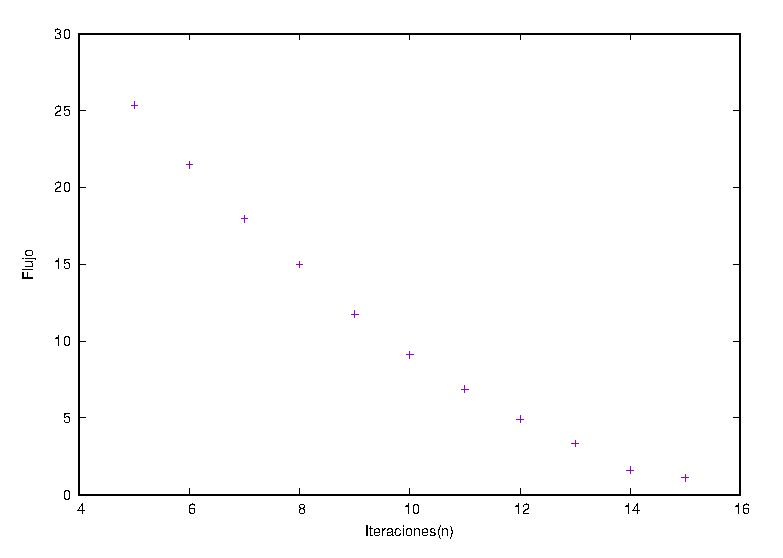
\includegraphics[scale=0.6]{Flujo-Iteraciones}
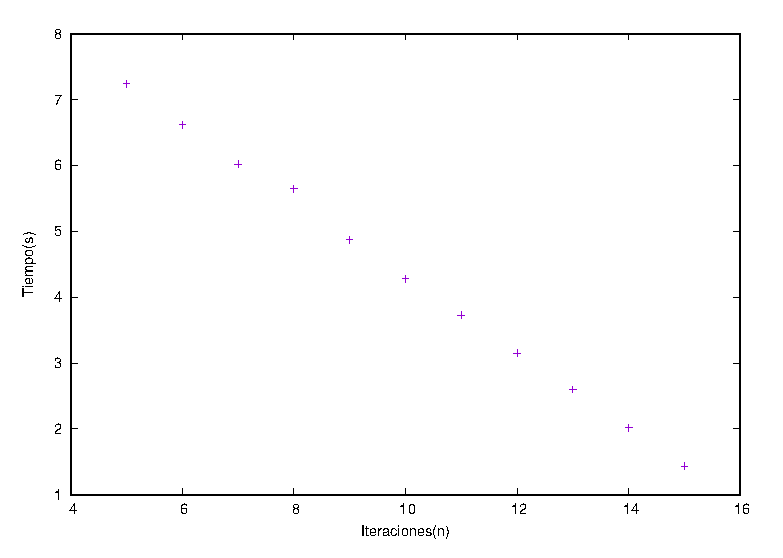
\includegraphics[scale=0.6]{Tiempo-Iteraciones}
\caption{\small A la izquierda la gráfica Flujo-Iteraciones, a la derecha la gráfica Tiempo-Iteraciones}
\end{figure}




\newpage

\begin{thebibliography}{a}

\bibitem{Python} \textit{Python versión 3} \url{https://www.python.org/}
\bibitem{Gnuplot} \textit{GNUPlot versión 5} \url{http://www.gnuplot.info/}
\bibitem{Tarea5} \textit{Tarea5.pdf} \url{https://github.com/SamatarouKami/OPTIMIZACION-DE-FLUJOS-DE-REDES/tree/master/Tarea5}
\bibitem{Contraccion} \textit{Contracción de Aristas} \url{https://es.wikipedia.org/wiki/Contracci%C3%B3n_de_aristas}
\bibitem{Ford-Fulkerson} \textit{Algoritmo Ford-Fulkerson} \url{https://es.wikipedia.org/wiki/Algoritmo_de_Ford-Fulkerson}
\bibitem{Resultados.dat} \textit{Resultados.dat} \url{https://github.com/SamatarouKami/OPTIMIZACION-DE-FLUJOS-DE-REDES/tree/master/Tarea6/Resultados.dat}
\end{thebibliography}

\end{document}